\begin{frame}{Conclusion}

    We have:
    \begin{itemize}
        \item Explored a Knowledge Graph-Based System (KGBS) architecture
        \item Detailed each KGBS containers and activities
        \item Explored a real-world use case moving from a text-based to a KG-based Information Retrieval (IR) System.
        \item Introduce and compared $3$ IR systems:
        \begin{itemize}
            \item A text-based IR system
            \item A concept-based IR system
            \item A KG-based IR system
        \end{itemize}
    \end{itemize}

     \begin{center}
        KG-based systems for IR on a multilingual corpus of technical documents show promising results overcoming the text-based approaches limitations.   
     \end{center}

\end{frame}

\begin{frame}{Future works}

    \begin{itemize}
        \item KGBS architecture:
        \begin{itemize}
            \item Implement an end-to-end Knowledge Graph-Based System architecture use case.
            \item Further explore the modularity of the architecture
        \end{itemize}
        \item Knowledge Graph-based Information Retrieval system:
        \begin{itemize}
            \item Expand the Knowledge Graph
            \item Enhance the concept matching task
            \item Expand the approach to other domains
        \end{itemize}
    \end{itemize}

\end{frame}

% \begin{frame}{Perspectives: Knowledge Graph}

%     \begin{figure} [H]
%         \begin{center}
%             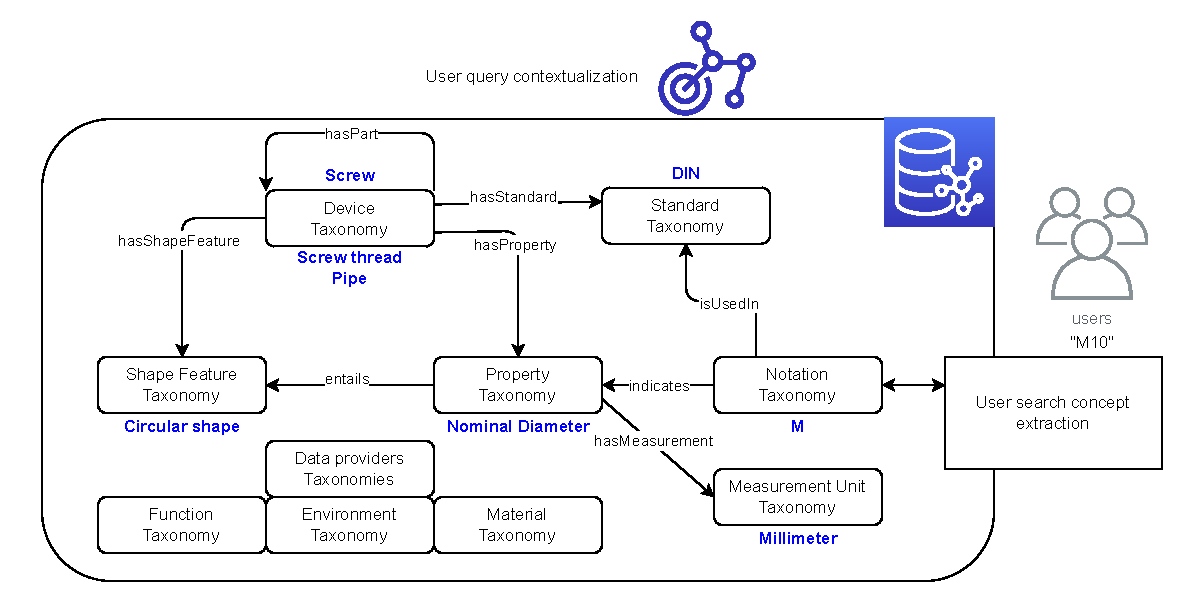
\includegraphics[scale=0.5]{images/semantic_search_example.pdf} 
%             \caption{Extended semantic search example.} 
%         \end{center}
%     \end{figure}

% \end{frame}

\begin{frame}{Contributions}

    % \begin{center}
    %     A top-down approach from a system perspective down to solution implementations.
    % \end{center}

    Main contributions:
    \begin{itemize}
        \item Ontology Learning Applied Framework (OLAF)
        \item An OWL Information Retrieval ontology
        \item Knowledge Graph-based Information Retrieval systems
    \end{itemize}

    Satellite contributions
    \begin{itemize}
        \item A unifying definition of Knowledge Graph
        \item An architecture for Knowledge Graph-Based Systems
    \end{itemize}
    
\end{frame}

\begin{frame}{Scientific productions}

    Peer-reviewed international conference papers:
    \begin{itemize}
        \item An operational architecture for knowledge graph-based systems. Proceedings of the 26th International Conference KES2022.
        \item (with Marion Schaeffer) Olaf: An ontology learning applied framework. Proceedings of the 27th International Conference KES2023.
    \end{itemize}

    Open-source software library (with Marion Schaeffer):
    \begin{itemize}
        \item Ontology Learning Applied Framework Python library implementation:\\\href{https://wikit-ai.github.io/olaf/}{https://wikit-ai.github.io/olaf/}
    \end{itemize}

\end{frame}